\chapter{Sicurezza dei Sistemi Operativi}
Un SO (Sistema Operativo), o OS (Operating System), gestisce il modo in cui le applicazioni software accedono alle risorse hardware del calcolatore:
\begin{itemize} 
  \item CPU
  \item Memoria principale
  \item Memoria secondaria
  \item Periferiche di I/O
  \item Interfacce di rete
\end{itemize}
Un OS fornisce un'interfaccia semplificata e consistente a utenti e applicazioni al fine di interagire con i componenti hardware. Grazie a questa astrazione è possibile sviluppare programmi software senza preoccuparsi della particolare tipologia di hardware sul quale saranno eseguiti. Gli OS svolgono numerose funzioni, alcune delle quali strettamente legate a problemi di sicurezza, in particolare vedremo:
\begin{itemize} 
  \item meccanismi di autenticazione
  \item sicurezza dei processi
  \item sicurezza del filesystem
  \item sicurezza della memoria
\end{itemize}
\section{Meccanismi di Autenticazione}
Un OS deve poter identificare i propri utenti in modo sicuro, i.e. utenti diversi potrebbero avere permessi di accesso alle risorse diversi. Un meccanismo di autenticazione standard ampiamente usato consiste nell'inserimento di un username e di una password: se la password inserita coincide con la password memorizzata dall'OS per il dato username allora l'utente viene autenticato. Un OS deve dunque memorizzare la password di ogni utente che può accedere al sistema. Generalmente gli OS memorizzano le password criptate attraverso funzioni hash in un file o in un apposito database. Grazie alla proprietà one-way delle funzioni hash, un attaccante che riesce ad accedere al file dove sono memorizzate le password non può ricostruire facilmente il loro valore. Tali file si trovano:
\begin{itemize} 
	  \item per Windows in \textit{C:\textbackslash WINDOWS \textbackslash system32 \textbackslash config \textbackslash SAM}
  \item per Linux in $/etc/passwd$ e in $/etc/shadow$ (solo l'utente root può leggerle)
\end{itemize}

\subsection{Possibili attacchi}
\begin{itemize} 
  \item \textbf{Brute Force}: attacco offline, tutte le possibili password per un dato alfabeto vengono generate automaticamente, criptate con la funzione hash usata dal sistema di autenticazione e confrontate con le password memorizzate
  \item \textbf{Dizionario}: attacco offline, liste di parole comuni (es: nomi) che vengono criptate con la funzione hash usata dal sistema di autenticazione e confrontate con le password memorizzate
  \item \textbf{Rainbow tables}
\end{itemize}
\subsection{Password Robuste}
Per la definizione di password robuste a tali attacchi vanno seguite delle ben definite linee guida:
\begin{itemize}
  \item evitare parole comuni (e.g. nomi)
  \item evitare password brevi
  \item usare caratteri maiuscoli E minuscoli
  \item usare caratteri speciali
  \item usare i numeri
\end{itemize}
Un esempio di password robusta è: "Voglio compr@re 11 Cani!": per scoprire questa password con un attacco brute-force in 60 giorni dovrei disporre di un computer in grado di generare circa $3,86 \cdot 10^{44} PW/sec$. Per rendere la struttura ancora più sicura si può impostare una scadenza alla password.
\subsection{Password Salt}
Il \textbf{Salt} consiste in una stringa di bit random da concatenare all'input di una funzione hash (o di un algoritmo di crittografia) al fine di aumentare la randomicità dell'output. Nel caso dell'autenticazione è possibile associare un numero random all'userID dell'utente, seguendo la forma: \newline \newline
\textbf{salt = numero random + userID} \newline \newline
\begin{figure}[htbp]
	\centering%
	\subfigure%
	{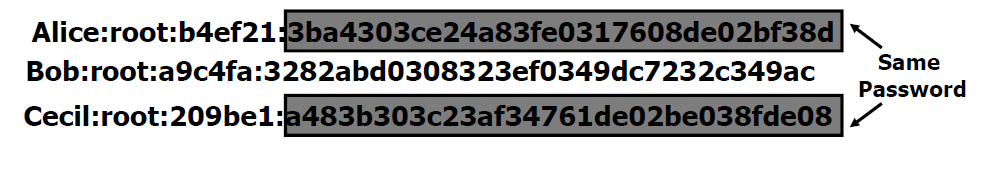
\includegraphics[height=8cm, width=13cm, keepaspectratio]{Immagini/sistemi_operativi/password.png}}
	\caption{Esempi di Salt \label{fig:salt}} 	
\end{figure}
\newpage
Il processo di autenticazione funziona nel seguente modo:
\begin{itemize}
  \item L'utente inserisce il suo userID X e la password P
  \item Il processo di autenticazione dell'OS recupera il salt S per l'userID X e l'hash H del salt concatenato alla password associata a X
  \item OS verifica se $HASH(S \vert \vert P) == H$
\end{itemize}
\begin{figure}[htbp]
	\centering%
	\subfigure%
	{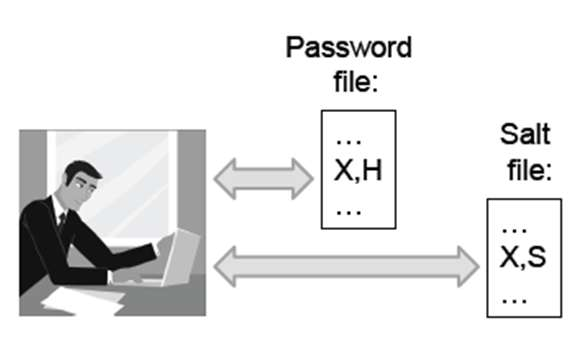
\includegraphics[height=8cm, width=8cm, keepaspectratio]{Immagini/sistemi_operativi/password2.png}}
	\caption{Processo di autenticazione con Salt \label{fig:salt}} 	
\end{figure}
Tale meccanismo comporta evidenti benefici. Se l'attaccante non può trovare il salt associato con l'userID, allora lo spazio di ricerca per un attacco con dizionario cresce notevolmente, diventando $2^{B} \cdot D$, dove B è il numero di bit del Salt, mentre D lo spazio del dizionario. \newline
Inoltre, anche se l'attaccante fosse in grado di recuperare il salt memorizzato in forma criptata dall'OS, questo meccanismo consente di rallentare notevolmente l'attacco con dizionario, rendendolo valido per un userID alla volta. Senza salt è possibile crackare molte password nello stesso momento, in quanto si ha solo bisogno dell'hash di ogni possibile password e di confrontarlo con tutti gli hash memorizzati. Con il meccanismo di salt, invece, ogni possibile password va
concatenata al salt ad essa associato prima di calcolarne l'hash.\\

Inoltre, è possibile che due utenti utilizzino la stessa password, o che lo stesso utente scelga di utilizzare la stessa password per due account diversi. Senza il meccanismo di salt le due password hanno lo stesso hash (questo potrebbe rivelare il fatto che i due account hanno la stessa password, permettendo a chiunque che conosce una delle due password di accedere anche all'altro account). Grazie al meccanismo di salt gli hash delle due password risultano invece diversi.

\section{Sicurezza dei processi}
Un processo è un'istanza di un programma in esecuzione: il codice di un programma in esecuzione viene caricato dalla memoria secondaria in cui è memorizzato e passato alla memoria primaria. Più istanze di uno stesso programma possono essere eseguite come processi diversi, e un'applicazione può essere composta da più di un processo.  I processi attivi vengono eseguiti "parallelamente" attraverso la tecnica di time-sharing su ogni core della CPU. Ogni processo è univocamente identificato da un intero detto \textbf{PID} (\textbf{P}rocess \textbf{ID} ) e viene associato all'user (utente) che lo ha generato. \newline 

Un processo può inoltre avviare e controllare altri processi. Un nuovo processo è generato mediante il meccanismo di \textbf{forking}. Il processo che richiede il forking è detto \textbf{parent process}, il processo forked è detto \textbf{child process}.
\begin{algorithm}
\begin{lstlisting}[caption={Esempio forking in C}]
int main()
{
	printf("I'm the parent, my PID is %d, my parent 
			is process %d\n", getpid(), getppid());
	fork();
	printf("This sentence has been printed by process:
	 		%d my parent is process %d\n", getpid(), 
	 		getppid());
}
\end{lstlisting}
\end{algorithm}
\subsection{Istruzione Fork}
L'istruzione fork() crea una copia del processo corrente. Tale funzione ritorna 0 nel processo figlio e un intero maggiore di 0 nel processo padre (il valore restituito è proprio il PID del figlio). Ritorna invece (al padre) un intero minore di 0 nel caso in cui non sia stato possibile creare un nuovo processo. Al momento del fork() viene creato un address space (porzione di memoria dedicata) separato per il processo figlio, il quale eredita una copia esatta di tutti i segmenti di memoria del processo padre (codice, stack, file descriptor, heap, variabili globali, e program counter).\newline

Il meccanismo di forking porta ad un'organizzazione dei processi rappresentabile con una struttura ad albero radicato (\textbf{rooted tree}). In Linux la radice dell'albero è sempre il processo \textbf{init} che viene lanciato dal kernel durante il processo di boot del sistema operativo. Il processo init crea poi nuovi processi. In Windows e applicazioni lanciate dagli utenti sono sempre figlie del processo \textbf{Windows Explorer}.

\subsection{Ulteriori nozioni sui processi - facoltativo}
\subsubsection{Comunicazione tra processi}
Esistono diversi meccanismi per la comunicazione tra processi:
\begin{itemize}
  \item lettura/scrittura di files: semplice ma inefficiente e poco sicuro
  \item porzione di memoria RAM condivisa. Questa soluzione è veloce e efficiente, ma il kernel deve gestire in maniera sicura la separazione tra porzioni di memoria condivise e private
  \item pipes e sockets: oggetti in RAM condivisi che fungono da canale virtuale tra due processi
  \item signals: notifiche asincrone, il processore interrompe il flusso del processo ricevente e verifica se esiste un gestore per la notifica (routine da eseguire)
\end{itemize}

\subsubsection{Demoni e Servizi}
\begin{itemize}
  \item \textbf{Linux}: i \textbf{daemons} sono processi lanciati prima dell'autenticazione dell'utente, tipicamente dal processo init. Tali processi possiedono permessi più alti di qualsiasi utente, sopravvivono al termine delle sessioni utente e sono indistinguibili dagli altri processi
  \item \textbf{Windows}: esistono processi analoghi chiamati \textbf{services}. Rispetto ai daemons sono distinguibili dagli altri processi, poiché sono monitorati in modo specifico all'interno del TaskManger (esistono due tab separati, uno per i processi e uno per i servizi)
\end{itemize}

\subsubsection{System Call}
I processi comunicano con il kernel per inoltrare le richieste verso l'hardware. La comunicazione avviene mediante librerie dette \textbf{system call}. Ad ogni system call segue generalmente un interrupt che vincola il processore a fermare l'esecuzione corrente e a gestire la chiamata. Possibili attacchi alla sicurezza degli OS prevedono la contraffazione di una system call al fine di eseguire codice malevolo ad ogni chiamata o danneggiamento di una system call al fine di compromettere il funzionamento del sistema. Sempre più spesso in realtà, i programmatori non usano direttamente le system call, ma delle API che fungono da strato intermedio tra le applicazioni e le system call, al fine di facilitare e migliorare la portabilità delle applicazioni. Le funzioni contenute in queste API invocano a loro volta opportune system call e spesso vi è una corrispondenza diretta tra una funzione API ed una corrispondente system call. Esistono tipi di System Call per ogni possibile operazione: controllo dei processi, gestione dei file, comunicazione fra processi, gestione dei dispositivi e gestione delle informazioni di sistema.

\subsection{Processi e Utenti}
Come già detto, ogni processo è associato ad un utente. Utenti specifici possono avere permessi maggiori rispetto agli utenti normali (e.g. installare o rimuovere programmi, modificare i permessi degli altri utenti, modificare la configurazione del sistema). \newline 

Nei sistemi Unix l'utente root non ha alcuna restrizione. Nei sistemi Windows esistono diversi utenti speciali: SYSTEM, LOCAL SERVICE e NETWORK SERVICE associati direttamente al sistema operativo, e uno o più utenti administrator. Laddove SYSTEM non ha restrizioni, administrator, LOCAL SERVICE e NETWORK SERVICE agiscono con permessi ridotti e specifici per i loro scopi. 

\subsubsection{Processi e Utenti - Linux}
In Linux ad ogni processo sono associati 4 indici:
\begin{itemize}
  \item un \textbf{uid} (user ID) che identifica l'utente che ha lanciato il processo
  \item un \textbf{gid} (group ID) che identifica il gruppo a cui appartiene l'utente
  \item un \textbf{euid} (effective user ID) che può differire dall'uid e identificare l'utente proprietario del file eseguibile, il quale può avere permessi maggiori. L'euid prevale sull'uid solo nel caso in cui è settato il bit \textbf{setuid}
  \item un \textbf{egid} (effective group ID) che può differire dal gid e identificare il gruppo proprietario dell'applicazione, il quale può avere permessi maggiori. L'egid prevale sul gid solo nel caso in cui è settato il bit \textbf{setgid}
\end{itemize}
Tramite questi id Linux è in grado di stabilire i permessi di un dato processo su una data risorsa. I permessi del processo figlio sono automaticamente ereditati dal processo padre.
\begin{algorithm}
\begin{lstlisting}[caption={Esempio forking in C}]
chmod u+s <file_eseguibile> %attiva setuid
chmod u-s <file_eseguibile> %disattiva setuid
chmod g+s <file_eseguibile> %attiva setgid
chmod g-s <file_eseguibile> %disattiva setgid
\end{lstlisting}
\end{algorithm}
Molti programmi che accedono risorse di sistema hanno il bit setuid settato e sono detti \textbf{setuid programs} (es: passwd, su). Questo meccanismo può essere soggetto ad attacchi di scalata dei privilegi, che vedremo più avanti. \newline 

Vediamo un esempio. Prendiamo un file eseguibile chiamato \textit{app}, con \textit{userA} e \textit{groupA} rispettivamente come UID e GID dell'utente proprietario del file e \textit{userB} e \textit{groupB} come UID e GID dell'utente che lancia app, producendo il processo \textit{P}. Se il bit SETUID di app è attivo, l'EUID di P è \textit{userA}, il EGID di P è \textit{groupA}. Se il bit SETUID di app non è attivo, EUID e UID coincidono con \textit{userB}, EGID e GID coincidono con \textit{groupB}. Supponiamo ora che il processo \textit{P} voglia accedere ad un file di nome \textit{info}. Se EUID di P coincide con il proprietario di \textit{info}, il processo acquisisce i diritti di accesso del proprietario di \textit{info}. Altrimenti se EGID di P e il gruppo di \textit{info} coincidono, P acquisisce i diritti di accesso del gruppo di utenti associato a \textit{info}. Se nessuna delle due precedenti condizioni è valida, valgono i normali diritti di accesso che vedremo più avanti (lettura/scrittura/esecuzione), l'accesso sarà consentito o meno a seconda della categoria di utenti nella quale ricadono UID e GID del processo P.

\section{Sicurezza del filesystem}
Il filesystem è un altro componente fondamentale di un OS, in quanto fornisce un'astrazione sull'organizzazione della memoria secondaria del calcolatore. Gli OS organizzano tipicamente i file in una gerarchia: ogni cartella può contenere file e/o sottocartelle. In questo modo è possibile rappresentare la memoria secondaria attraverso una struttura ad albero radicato. Prima di affrontare il tema della sicurezza del filesystem, diamo due definizioni:
\begin{itemize}
  \item \textbf{Principal}: utente o gruppo di utenti
  \item \textbf{Permission}: azione possibile (e.g.: read, write, execute, list)
\end{itemize}

\subsubsection{Access Control Entries}
Una \textbf{Access Control Entry, ACE,} è una terna $\langle principal, type, permission \rangle$, che definisce esplicitamente cosa è possibile fare e cosa non per una specifica risorsa e per un dato principal. Il campo \textbf{type} può assumere due valori: \textbf{allow} o \textbf{deny}. \newline 

Una \textbf{Access Control List} è invece una lista ordinata di terne \textbf{ACE}. Una possibile gestione per la sicurezza del filesystem prevede l'associazione di una ACL ad ogni file e directory in modo da definire la politica di accesso alla risorsa.

\subsubsection{Discretionary Access Control}
Il \textbf{DAC (Discretionary Access Control)} è un modello di assegnazione dei permessi in cui il creatore (owner) di un file o directory ha il potere di modificare i permessi ad esso associati (ACE). Sono disponibili due tipi di politiche di assegnazione dei permessi:
\begin{itemize}
  \item \textbf{Closed policy o default sicuro}: solo ACE di tipo allow, tutti i permessi non esplicitamente concessi sono automaticamente negati
  \item \textbf{Open policy}: ACE tipo sia ALLOW che DENY
\end{itemize}

\subsection{Sicurezza del filesystem Linux}
Per la gestione dei permessi, Linux utilizza una politica \textbf{DAC} con \textbf{default sicuro}. Inoltre l'accesso a un file dipende dall'ACL del file e di tutte le directory antenate: partendo dalla directory root, tutte le directory antenate devono avere il permesso \textbf{execute} (che per una directory significa il permesso di accedere alla stessa) per l'utente specificato. \newline

Linux utilizza una versione semplificata delle ACL: la \textbf{File permission matrix}, una matrice di permessi associata ad ogni file e directory (tale metodologia rappresenta uno standard per tutti i sistemi Unix-like). La matrice presenta tre principal: \textbf{owner}, \textbf{group} (utenti del gruppo a cui afferisce l'owner) e \textbf{others}. I permessi di ognuna delle 3 classi sono definiti da 3 bit:
\begin{itemize}
  \item \textbf{read bit}: per i file rappresenta il permesso di lettura, mentre per le directory il permesso di lettura della lista dei file contenuti
  \item \textbf{write bit}: per i file rappresenta il permesso di scrittura, mentre per una directory il permesso di creazione e eliminazione dei file in essa contenuti
  \item \textbf{execute bit}: per i file rappresenta il permesso di esecuzione, mentre per le directory il permesso di accesso (l'utente può cambiare la sua cartella corrente con quella in questione)
\end{itemize}

\begin{figure}[htbp]
	\centering%
	\subfigure%
	{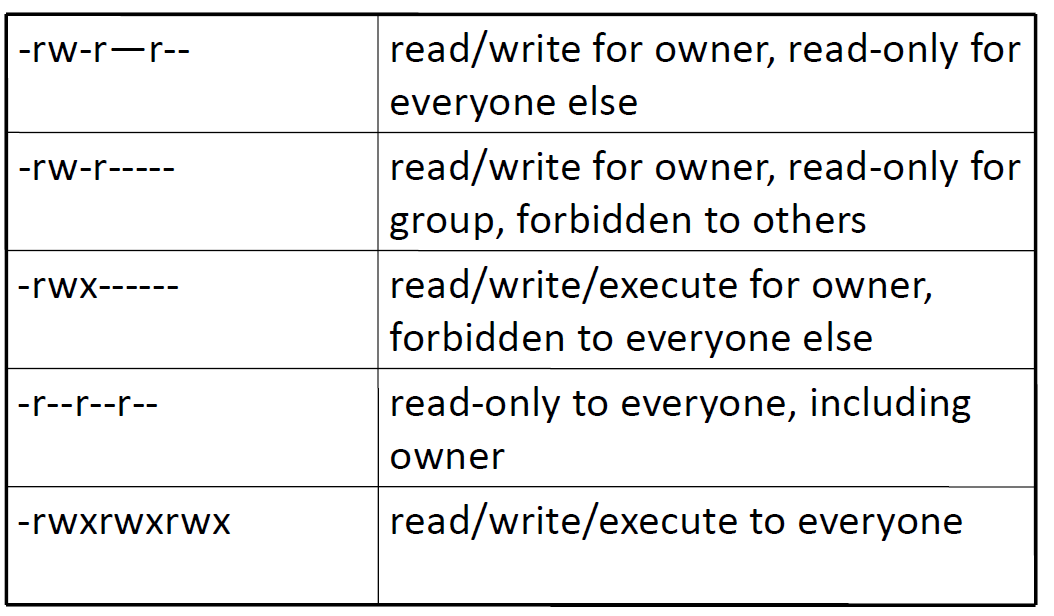
\includegraphics[height=10cm, width=10cm, keepaspectratio]{Immagini/sistemi_operativi/perm_linux.png}}
	\caption{Esempi di permission matrix \label{fig:perm_linux}} 	
\end{figure}

Per visualizzare le permission matrix delle directory e dei file contenuti in una directory, basta accedere a tale cartella e utilizzare il comando \textbf{ls -l}. \newline \newline

Oltre ai tipi di permessi esaminati finora, esistono altri tipi di permessi cosiddetti \textbf{speciali}, i quali consentono di impostare determinate funzioni avanzate sui file.

\begin{itemize}
  \item \textbf{Set-user-ID (suid o setuid) bit}: su file eseguibili, causa l'esecuzione del processo con i diritti dell'utente owner
  \item \textbf{Set-group-ID (sgid o setgid) bit}: su file eseguibili, causa l'esecuzione del processo con i diritti del gruppo del file
  \item \textbf{Sticky bit}: sulle directory, vieta a tutti gli utenti di eliminare o rinominare file di cui non sono i creatori
\end{itemize}

Il bit \textbf{setuid} risolve il problema dell'accesso senza privilegio. Ad esempio, se un utente volesse modificare la propria password attraverso il programma di sistema \textbf{passwd} non potrebbe farlo in quanto non avrebbe i permessi per accedere al file \textbf{etc/passwd}. In realtà \textbf{passwd} viene eseguito con i privilegi dell'utente root grazie al bit setuid.

\subsubsection{Scalata dei privilegi}
Se un attaccante riesce a forzare un \textbf{programma setuid} a eseguire codice arbitrario (ad esempio tramite un attacco di tipo buffer overflow) può compromettere il sistema, realizzando uno scenario di attacco chiamato \textbf{scalata dei privilegi (o privileges escalation)}. Questo meccanismo va gestito attraverso tecniche di programmazione sicura.

\subsubsection{Notazione Ottale}
Nei sistemi Linux i bit di permessi sono espressi in notazione ottale (con 3 o 4 cifre). Le cifre sono organizzate nel seguente modo: \newline
\textbf{[special bits][user bits][group bits][others bits]}. Ogni sezione deve prevedere ovviamente tre bit: uno per la scrittura, uno per la lettura ed uno per l'esecuzione. 

\begin{figure}[htbp]
	\centering%
	\subfigure%
	{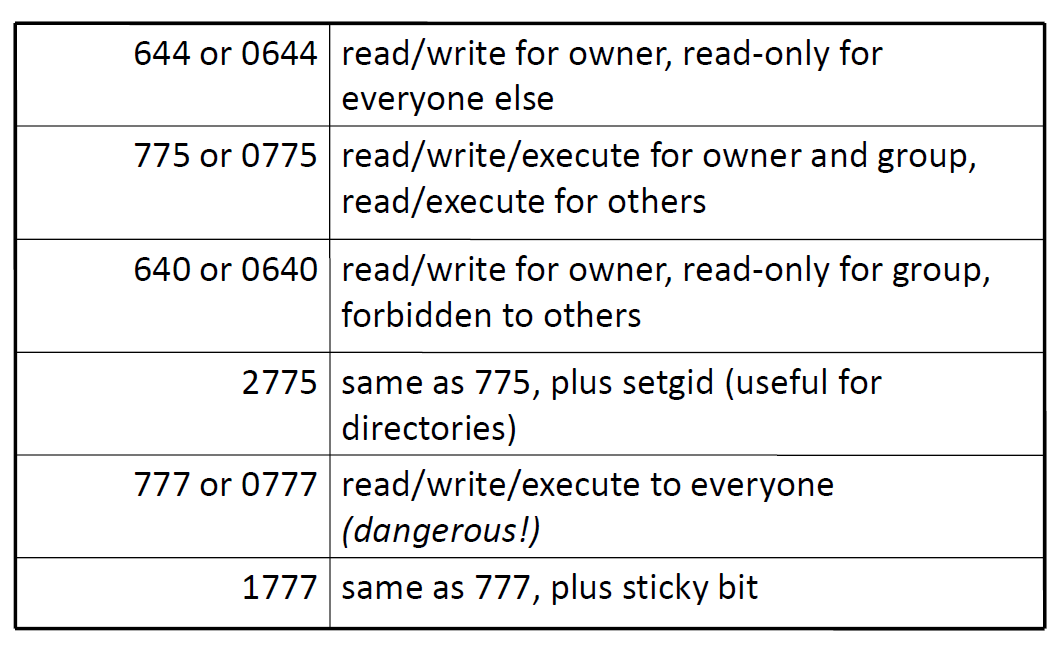
\includegraphics[height=10cm, width=10cm, keepaspectratio]{Immagini/sistemi_operativi/notazione_ottale.png}}
	\caption{Esempi di permission matrix in notazione ottale\label{fig:notazione_ottale}} 	
\end{figure}
\begin{itemize}
  \item per i bit user/group/others, i bit sono nell'ordine r-w-x. Una terna $(100)_{2} = (4)_{8}$, ad esempio, significa permesso consentito in lettura, mentre una terna $(101)_{2} = (5)_{8}$, invece, permesso consentito in lettura ed esecuzione, ma non in scrittura.
  \item per i speciali, i bit sono nell'ordine setuid - setgid - sticky. Quindi avrò $(100)_{2} = (4)_{8}$ se setuid, $(010)_{2} = (2)_{8}$ se setgid e $(001)_{2} = (1)_{8}$ se sticky (e ovviamente le varie combinazioni possibili)
\end{itemize}

\subsection{Sicurezza del filesystem Windows}
Per la gestione dei permessi Windows utilizza una politica \textbf{DAC} con \textbf{open policy}. Se non c'è una regola per un particolare principal o permesso allora l'accesso è negato di default. A differenza di Linux, al fine di accedere ad un file o ad una directory, è sufficiente avere i permessi per l'azione richiesta sul dato file o directory. In questo modo è possibile negare l'accesso ad una data directory pur consentendo l'accesso alle directory figlie.\newline 

Vi sono due tipi di permessi: espliciti ed ereditati. Il concetto di \textbf{permessi ereditati} deriva dalla possibilità di estendere ogni permesso applicato ad una directory alle directory figlie. I \textbf{permessi espliciti} standard sono: \emph{modify, read and execute, read, write, full control}. E' possibile comporre più \textbf{permessi standard} creando \textbf{permessi avanzati}. \\ \\
Per quanto riguarda il controllo dei permessi va notato che:
\begin{itemize}
  \item Il permesso DENY ha precedenza sul permesso ALLOW
  \item I permessi espliciti hanno precedenza sui permessi ereditati
  \item I permessi ereditati hanno precedenza tra di loro in base alla distanza dalla risorsa
\end{itemize}
  
\subsubsection{File Descriptors e File Handles}
Un \textbf{file descriptor}, per Unix, o \textbf{file handle}, per Windows, è un identificatore per un file, una pipe o un socket aperto da un processo e sul quale il processo può effettuare operazioni di input/output. I file descriptor sono memorizzati in una tabella che li mappa con il percorso del file a cui si riferiscono, chiamata \textbf{file descriptor table}. L'accesso ai file e cartelle tramite System Calls passa quindi per questi costrutti. Le operazioni possibili sono:
\begin{itemize}
  \item \textbf{open}: ritorna un file handle
  \item \textbf{read/write/execute} file
  \item \textbf{close} file: invalida il file handle
\end{itemize}
Quando un processo (programma) necessita di accedere ad un file in lettura o scrittura: viene richiamata la \textbf{system call open}. Il kernel verifica se il processo possiede i permessi necessari per accedere al file con l'azione richiesta e, se la verifica è positiva, crea un nuovo file descriptor e una nuova entry nella file descriptor table, quindi ritorna il file descriptor al processo. Il processo può leggere/scrivere sul file richiamando le relative system call read/write, e il kernel (attraverso la file descriptor table) effettua le letture/scritture direttamente sul file originale. Al termine dell'elaborazione del file il processo dovrebbe richiamare una close system call
per rimuovere il file descriptor.

\subsubsection{File Descriptors Leaks}
Quando un processo crea un processo figlio (forking), quest'ultimo eredita una copia di tutti i file descriptors aperti dal processo padre. L'OS verifica i permessi soltanto al momento della creazione del file descriptor: al momento della lettura/scrittura sul file, i controlli effettuati si basano sui permessi associati al file descriptor (ad esempio un processo può sfruttare un file descriptor in lettura solo per leggere il file e non per scrivere). Un possibile scenario pericoloso potrebbe presentarsi nel caso che un processo con alti privilegi apra un file descriptor per un file protetto, prima di chiudere il file descriptor crei un nuovo processo con privilegi minori, il quale tuttavia erediterebbe comunque il file descriptor (in quanto ancora aperto). In tal caso, infatti, il processo figlio potrebbe usare il file descriptor pur non avendo i permessi necessari per operare sul file protetto.

\begin{algorithm}
\begin{lstlisting}
[caption={Esempio codice vulnerabile al File Descriptors Leaks]
#include <stdio.h>
#include <unistd.h>
int main(int argc, char * argv[ ])
{
	/* Open the password file for reading */
	FILE *passwords;
	passwords = fopen("/home/admin/passwords", "r");
	/* Read the passwords and do something useful */
	/* . . . */
	/* Fork and execute Joe's shell without closing the file */
	execl("/home/joe/shell", "shell", NULL);
}
\end{lstlisting}
\end{algorithm}
Per rimuovere questa vulnerabilità la funzione \textbf{fclose()} va richiamata prima del comando \textbf{execl()}.

\section{Sicurezza della memoria}
Un ulteriore servizio offerto dagli OS è l'organizzazione e l'allocazione della memoria primaria. Quando un processo viene lanciato l'OS alloca una regione di memoria detta \textbf{address space} del processo. La gestione della memoria è trasparente per il processo: il processo “vede” a sua disposizione l'intera memoria. Generalmente un processo non può avere accesso all'address space di un altro processo, se non per risorse esplicitamente condivise. \\ \\
Nei sistemi Unix-like il modello address space è diviso in 5 settori:
\begin{itemize}
  \item \textbf{Text}: memorizza il codice macchina del programma
  \item \textbf{Data}: memorizza le variabili statiche del programma inizializzate prima dell'esecuzione
  \item	\textbf{BSS (Block Started By Symbol)}: memorizza le variabili statiche del programma non inizializzate
  \item	\textbf{Heap}: settore dinamico, memorizza i dati generati durante l'esecuzione del programma (es: oggetti Java/C++) 
  \item	\textbf{Stack}: memorizza una struttura dati a pila, che tiene traccia delle chiamate a metodi e routine con i relativi argomenti e punti di ritorno 
\end{itemize}
In \figurename~\ref{fig:addr_space_unix} è mostrato il modello. Si noti che lo Stack cresce verso il basso. In tale modello ogni settore ha i suoi permessi: il settore text è read-only in quanto il codice macchina del programma in esecuzione non deve poter essere modificato, mentre gli altri settori necessitano di essere writable in quanto i loro dati devono poter essere modificati durante l'esecuzione.
\begin{figure}[htbp]
	\centering
	\subfigure
	{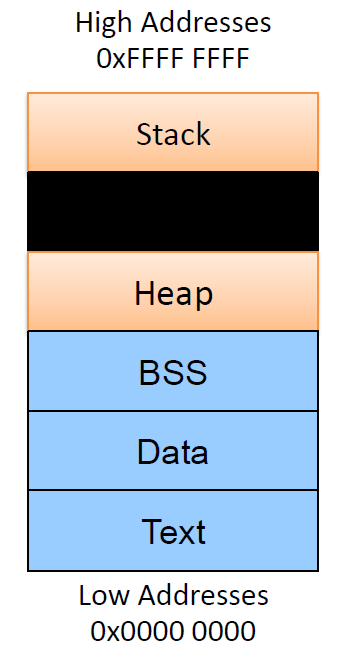
\includegraphics[height=10cm, width=13cm, keepaspectratio]{Immagini/sistemi_operativi/addr_space_unix.png}}
	\caption{Modello Address Space Unix \label{fig:addr_space_unix}} 	
\end{figure}

\section{Exploit}
Un \textbf{exploit} è un input che sfrutta una vulnerabilità, un bug o un guasto di un sistema al fine di eseguire un attacco. Una metodologia tipica di attacco prevede:
\begin{itemize}
  \item la ricerca di una vulnerabilità
  \item reverse engineering del codice
  \item	costruzione dell'exploit
\end{itemize}

\subsection{Buffer Overflow}
Generalmente, con \textbf{buffer}, si intende una porzione contigua di memoria contenente più istanze dello stesso tipo. In C e in molti altri programmi i buffer sono chiamati array. I buffer più comuni sono gli array di caratteri (stringhe).
In C i buffer, come tutte le variabili, possono essere dichiarati statici o dinamici. Le variabili statiche sono allocate al momento del caricamento del programma sul segmento \textbf{data}, mentre le variabili dinamiche sono allocate in fase di esecuzione sullo \textbf{stack}. \newline 

\subsubsection{Scenario}
Un programma alloca in memoria un buffer (array) di dimensione fissata. Nel buffer viene poi copiato un input proveniente dall'utente, e la dimensione di tale input \textbf{non viene controllata} prima dell'operazione di copia.

\subsubsection{Attacco}
Un attaccante può confezionare un input malevolo di dimensione superiore a quella del buffer. Il programma copia l'input e sovrascrive regioni di memoria oltre al buffer. L'attaccante riesce a eseguire codice malevolo (\textbf{shellcode}) con i privilegi del programma attaccato. Il buffer riempito di codice malevolo viene denominato \textbf{payload}. L'attaccante solitamente inietta codice in grado di aprire un terminale (shell) attraverso cui eseguire altri comandi (e.g. Linux: /bin/sh, Windows: command.com). Ad esempio in un sistema Linux è possibile iniettare codice che richiama la funzione \textbf{setuid()} per poi aprire un terminale. Il codice viene generalmente iniettato direttamente sullo stack o sull'heap e pertanto deve essere scritto in codice operativo (\textbf{opcodes}) specifico per l'architettura della CPU attaccata.

\subsection{Stack-Based Buffer Overflow}
I moderni computer sono progettati tenendo in mente la necessità di poter usufruire di linguaggi di alto livello (con caratteristiche di \textbf{programmazione strutturata}, come C e C++). La tecnica più importante per la strutturazione dei programmi introdotta dai primi linguaggi di alto livello è la routine (function). Una chiamata a una procedura altera il flusso di controllo proprio come fa un salto, ma a differenza di un salto, al suo termine il controllo ritorna alla dichiarazione o istruzione successiva alla chiamata. Questo alto livello di astrazione è implementato con l'aiuto dello stack. Lo stack è infatti usato nell'ambito delle routine per allocare dinamicamente le variabili locali, per il passaggio dei parametri, e per la restituzione di valori. \newline

Lo stack è un settore dell'address space contenente dati. La sua dimensione è regolata dinamicamente dal kernel
in fase di esecuzione, tramite una politica LIFO e opportune chiamate a funzioni push/pop. Ogni chiamata ad una routine è associata ad un frame che memorizza le variabili locali, gli argomenti, e l'indirizzo di ritorno verso la chiamata padre. Alla base dello stack c'è quindi il frame relativo alla chiamata main(). Un buffer overflow che coinvolge una variabile locale può causare la sovrascrittura di parte della memoria allocata nello stack, con conseguenze pericolose. \\ \\
Lo stack viene gestito attraverso opportune variabili e registri (vedi \figurename~\ref{fig:stack_struct}):
\begin{itemize}
  \item \textbf{Return address:} puntatore all'indirizzo di memoria in cui la routine in questione è stata chiamata
  \item \textbf{Stack Pointer (ESP):} registro dedicato che contiene l'indirizzo dell'ultima locazione di memoria occupata sullo stack (ovvero il top dello stack vista la politica LIFO di inserimento). Viene aggiornato continuamente vista la dinamicità dello stack
  \item \textbf{Frame pointer (EBP)}: registro per tenere traccia della prima locazione di memoria del record di attivazione di una routine
\end{itemize}
\begin{figure}[htbp]
	\centering%
	\subfigure%
	{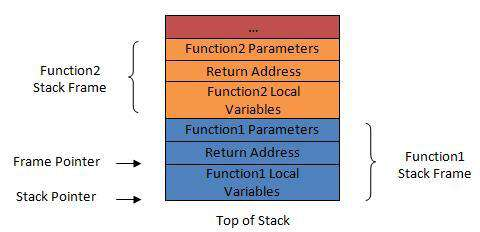
\includegraphics[height=13cm, width=13cm, keepaspectratio]{Immagini/sistemi_operativi/buffer.png}}
	\caption{Stack Structure \label{fig:stack_struct}} 	
\end{figure}
Gli indirizzi delle variabili locali di una routine sono specificati rispetto al frame pointer poiché il suo valore rimane invariato per tutta la durata della routine stessa. \newline \newline
\begin{figure}[htbp]
	\centering%
	\subfigure%
	{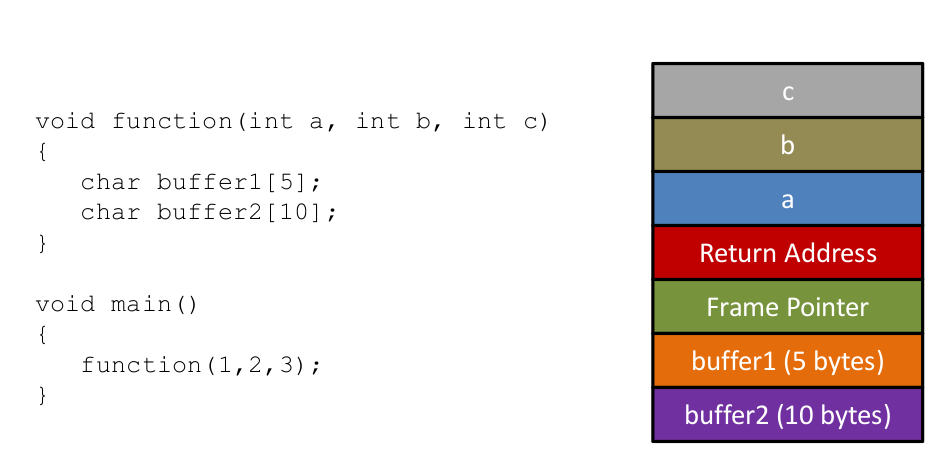
\includegraphics[height=13cm, width=13cm, keepaspectratio]{Immagini/sistemi_operativi/esempio_stack.png}}
	\caption{Esempio Stack di un programma in C\label{fig:esempio_stack}} 	
\end{figure}
\subsection{Esempio codice C}
Prendiamo come esempio la funzione \textit{strcpy(dest,src)}. Tale funzione (appartenente alle librerie standard del C) copia la stringa \textit{src} in \textit{dest} senza verificare se la dimensione di \textit{src} eccede quella di \textit{dest}. Per rimediare a questa vulnerabilità basta utilizzare la funzione \textit{strncpy(dest,src,n)}, che consente di specificare il numero di caratteri da copiare, e se la lunghezza di src supera tale soglia i caratteri in eccesso vengono scartati.
\begin{algorithm}
\begin{lstlisting}[caption={Esempio codice vulnerabile al buffer overflow in C}]
Main(int argc, char *argv[])
/* get user_input */
{
	char var1[15];
	char command[20];
	strcpy(command, "whois");
	strcat(command, argv[1]);
	strcpy(var1, argv[1]);
	printf(var1);
	system(command);
}
\end{lstlisting}
\end{algorithm}
\begin{figure}[htbp]
	\centering%
	\subfigure%
	{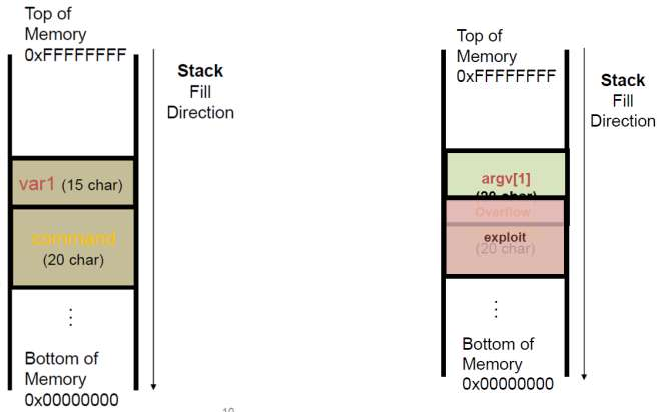
\includegraphics[height=7cm, width=13cm, keepaspectratio]{Immagini/sistemi_operativi/esempio_stack_2.png}}
	\caption{Esempio Stack-Based buffer overflow\label{fig:esempio_stack}} 	
\end{figure}

\subsection{Stack Smashing Attack}
In questo tipo di exploit l'attaccante sfrutta una vulnerabilità buffer overflow per sovrascrivere l'indirizzo di ritorno della routine corrente. Quando la routine termina il programma esegue il codice malevolo iniettato dall'attaccante, anziché riprendere il normale flusso di esecuzione. La difficoltà di quest'attacco consiste nel fatto che l'attaccante deve conoscere l'esatta posizione sullo stack dell'indirizzo di ritorno. Al fine di confezionare un attacco efficace l'attaccante deve, infatti:
\begin{itemize}
  \item assicurarsi che il codice malevolo iniettato risieda nell'address space del processo attaccato (altrimenti non sarebbe eseguito). Il codice può essere tenuto nel buffer stesso (payload)
  \item conoscere l'indirizzo esatto del codice malevolo
  \item e riuscire a sovrascrivere l'indirizzo di ritorno con l'indirizzo del codice malevolo
\end{itemize}
Per svolgere quest'ultimo task sono disponibili diverse tecniche, che vedremo nei paragrafi seguenti.
\begin{figure}[htbp]
	\centering%
	\subfigure%
	{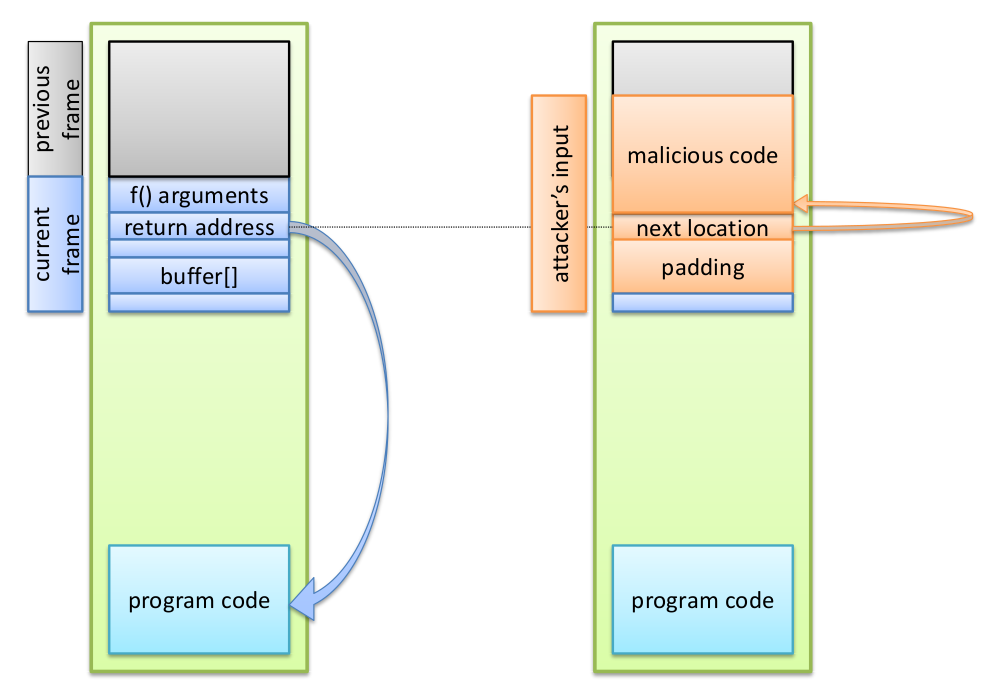
\includegraphics[height=13cm, width=13cm, keepaspectratio]{Immagini/sistemi_operativi/stack_smash.png}}
	\caption{Esempio Stack-Smashing\label{fig:stack_smash}} 	
\end{figure}
\subsection{NOP Sledding}
Al fine di semplificare la stima dell'indirizzo del codice malevolo (da posizionare nel return address dello stack) si può incrementare la dimensione del payload inserendo un gran numero di operazione \textbf{NOP (No-OP)}. Un'istruzione di questo tipo non fa nulla e il processore passa all'istruzione seguente. Se l'attacco funziona il processo salterà al punto di ritorno stimato (sovrascritto da qualche operazione NOP) e "slitterà" attraverso le istruzioni NOP verso il codice malevolo. L'attaccante deve confezionare quindi un input che contiene:
\begin{itemize}
  \item una quantità di dati appropriata da eccedere le dimensioni del buffer
  \item una stima dell'indirizzo di ritorno
  \item una grande quantità di istruzioni NOP
  \item lo shellcode
\end{itemize}
\begin{figure}[htbp]
	\centering%
	\subfigure%
	{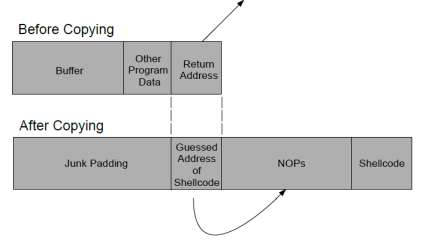
\includegraphics[height=13cm, width=13cm, keepaspectratio]{Immagini/sistemi_operativi/nop_sledding.png}}
	{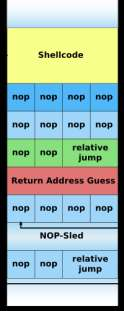
\includegraphics[height=10cm, width=13cm, keepaspectratio]{Immagini/sistemi_operativi/nop_sledding_2.png}}
	\caption{NOP Sledding\label{fig:nop_sledding}} 	
\end{figure}
Il NOP-Sledding aumenta le probabilità di riuscita per un attacco buffer overflow. E' un attacco molto utilizzato, anche se presenta ancora diverse difficoltà: è difficile da automatizzare, serve molto spazio per il payload e bisogna ancora stimare, in qualche misura, l'indirizzo dello shellcode.
\subsection{Trampolining}
Questo tipo di attacco sfrutta la previdibilità dell'allocazione nella memoria di librerie esterne. Al momento della loro inizializzazione molti processi caricano in zone protette del loro address space tali librerie. Un attaccante può sfruttare la conoscenza di una libreria di sistema per eseguire un attacco senza dover conoscere l'indirizzo dello shellcode. Ad esempio, se si è a conoscenza che una DLL di Windows richiede al processore di saltare all'indirizzo contenuto nel registro ESP che punta ad un buffer, si può inserire del codice malevolo nel buffer indirizzato dal registro e sovrascrivere il punto di ritorno della funzione corrente con quello dell'istruzione nota della DLL. E' un attacco abbastanza complesso, ma molto pericoloso in quanto automatizzabile.
\subsection{Return to libc}
Anche questa tecnica sfrutta librerie esterne caricate in fase di esecuzione. In questo caso vengono utilizzate le librerie C, chiamate \textbf{libc}. L'idea consiste nel determinare l'indirizzo di una funzione presente nelle librerie C all'interno dell'address space da colpire e forzare il programma a chiamare questa funzione. Nelle librerie C esistono diverse funzioni vulnerabili a questo tipo di attacco (e.g. exec(), system()).
L'attacco consiste nel:
\begin{itemize}
  \item sovrascrivere l'indirizzo di ritorno della funzione corrente con la funzione di libc da richiamare 
  \item sovrascrivere il buffer con gli argomenti per la funzione chiamata (e.g. con $"bin/sh"$)
\end{itemize}
\begin{figure}[htbp]
	\centering%
	\subfigure%
	{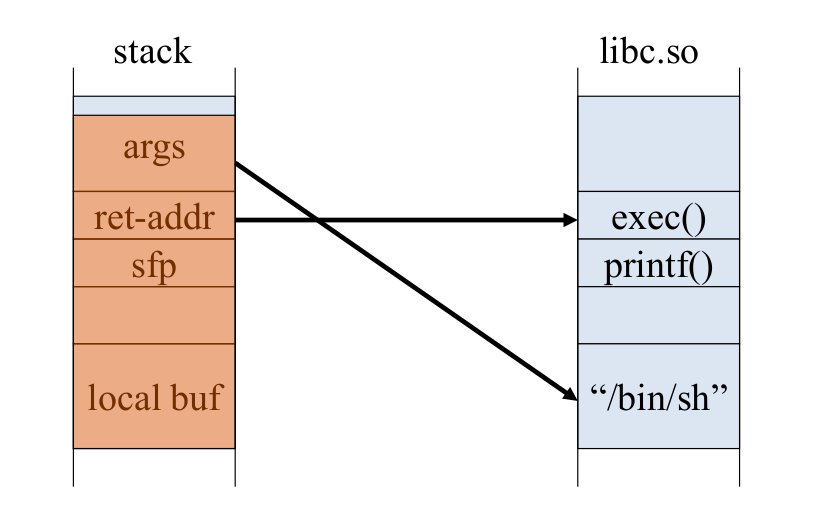
\includegraphics[height=13cm, width=13cm, keepaspectratio]{Immagini/sistemi_operativi/return_libc.png}}
	\caption{Esempio return to libc\label{fig:return_libc}} 	
\end{figure}
Il principale vantaggio di questa tecnica consiste nel fatto che non viene eseguito alcun codice sullo stack, rendendo inefficaci le contromisure che rendono lo stack non eseguibile.

\subsection{Contromisure Stack-Based BO}
\begin{itemize}
  \item Scrivere codice sicuro che verifica sempre le dimensioni dell'input proveniente dall'utente 
  \item Utilizzare linguaggi di programmazione che non consentono questo tipo di attacchi. \textit{C} e \textit{C++} sono vulnerabili, mentre $Java$, ad esempio, no, poiché gli oggetti vengono allocati dinamicamente sullo heap.
  \item Utilizzare meccanismi di protezione a livello di OS, come vedremo nei seguenti paragrafi
\end{itemize}
\subsubsection{No eXecute bit - NX bit}
Una possibile contromisura a questo tipo di attacchi è l'introduzione di un bit che marca i segmenti di memoria relativi allo stack e all'heap. In questo modo non è possibile eseguire shellcode direttamente in queste porzioni di memoria. Come accennato nel paragrafo precedente, questa contromisura \textbf{non} è efficace contro attacchi del tipo \textbf{return-to-libc}.
\subsubsection{Address Space Layout Randomization - ASLR}
Tecnica che consiste nell'arrangiare randomicamente l'address space di un processo. Ad esempio, due boot di Windows Vista danno luogo a locazioni delle librerie in memoria diverse, come mostrato in \figurename~\ref{fig:aslr}.
\begin{figure}[htbp]
	\centering%
	\subfigure%
	{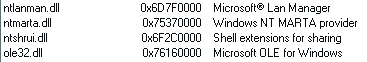
\includegraphics[height=13cm, width=10cm, keepaspectratio]{Immagini/sistemi_operativi/aslr.png}}
	{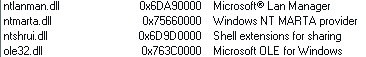
\includegraphics[height=13cm, width=10cm, keepaspectratio]{Immagini/sistemi_operativi/aslr_2.png}}
	\caption{Effetto ASLR sull'indirizzo di librerie Windows\label{fig:aslr}} 	
\end{figure}
\subsubsection{Stack-Smashing protection}
Tecnica che prevede un controllo in fase di esecuzione. Nel momento in cui una routine chiama l'indirizzo di ritorno l'OS verifica che lo stack non sia stato
modificato rispetto al momento in cui la funzione è stata chiamata. Se lo stack è stato modificato viene lanciato un errore di tipo \textbf{segmentation fault} e il programma termina forzatamente.
\subsubsection{Canary}
Anche questo metodo implementa un controllo in fase di esecuzione. Si definisce \textbf{Canary} un valore di controllo (spesso randomico) inserito dall'OS dopo un buffer o prima dell'indirizzo di ritorno. L'OS verifica regolarmente l'integrità di questo valore: in caso di buffer overflow viene sovrascritto anche il Canary, allertando l'OS.
\begin{figure}[htbp]
	\centering%
	\subfigure%
	{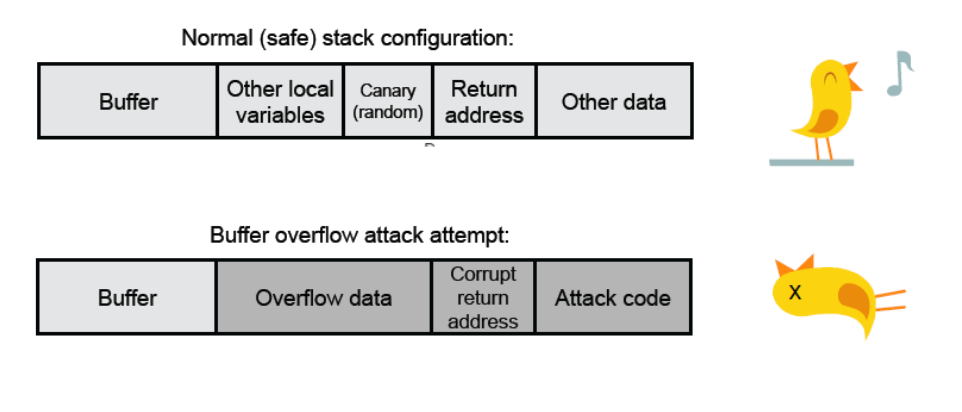
\includegraphics[height=13cm, width=13cm, keepaspectratio]{Immagini/sistemi_operativi/canary.png}}
	\caption{Canary\label{fig:canary}} 	
\end{figure}
\subsection{Race Conditions}
Una race condition è una situazione in cui il comportamento del programma è (involontariamente) dipendente dalla tempistica in cui si verificano certi eventi. Un classico esempio di queste situazioni fa uso delle seguenti due funzioni C:
\begin{itemize}
  \item la funzione \textbf{open()} apre il file specificato utilizzando l'userID effettivo (piuttosto che l'userID reale) del processo chiamante per verificarne i permessi. In altre parole, se un programma setuid di proprietà dell'utente root è lanciato da un utente normale, il programma può chiamare con successo open() sui file per i quali solo l'utente root ha il permesso di accedere
  \item la funzione \textbf{access()} controlla se l'utente reale (in questo caso l'utente che esegue il programma) ha permesso di accedere al file specificato
\end{itemize}
Analizziamo ora l'esempio in questione. Supponiamo che un semplice programma richieda il nome di un file come argomento, controlli se l'utente che esegue il programma ha il permesso di aprire il file e in caso affermativo legga i primi caratteri del file e li stampi. C'è una race condition in questa implementazione:  vi è un piccolo delay tra le chiamate ad access() ed a open(). Un utente malintenzionato potrebbe sfruttare questo piccolo ritardo, modificando il file in questione tra le due chiamate.
\begin{algorithm}
\begin{lstlisting}[caption={Esempio codice vulnerabile a race conditions}]

#include <stdio.h>
#include <string.h>
#include <stdlib.h>
#include <sys/types.h>
#include <fcntl.h>

int main(int argc, char * argv[ ])
{
	int file;
	char buf[1024];
	memset(buf, 0, 1024);
	if(argc < 2) {
		printf("Usage: printer [filename]\n");
		exit(-1);
	}
	
	if(access(argv[1], R_OK) != 0) {
		printf("Cannot access file.\n");
		exit(-1);
	}
	
	file = open(argv[1], O_RDONLY);
	read(file, buf, 1023);
	close(file);
	printf("%s\n", buf);
	return 0;
}

\end{lstlisting}
\end{algorithm}

Ad esempio, supponiamo che l'attaccante richieda /home/joe/dummy come argomento, un file di testo innocente a cui egli può accedere. Dopo che la chiamata access() restituisce 0, indicando che l'utente dispone dell'autorizzazione per accedere al file, l'utente malintenzionato può sostituire rapidamente /home/joe/dummy con un link simbolico a un file di cui non ha l'autorizzazione in lettura, come /etc/passwd. Successivamente, il programma chiamerà open() sul link simbolico, che avrà successo perché il programma setuid ha come proprietario
root. \\

Si noti che questo tipo di attacco non potrebbe essere fatto manualmente: la differenza di tempo tra due chiamate di funzione è abbastanza piccola da fare in modo che nessun essere umano sia in grado di modificare il file in tempo. E’ invece possibile avere un programma in esecuzione in background che scambia più volte i due file, ed esegue il programma vulnerabile finché lo scambio non si verifica esattamente tra le due istruzioni open() e access().

\subsubsection{Time of Check/Time of Use Problem}
In generale, questo tipo di vulnerabilità è conosciuto come Time of Check/Time of Use (\textbf{TOCTOU}) problem. Ogni volta che un programma controlla la validità e la le autorizzazioni per un oggetto, sia esso un file o di qualche altra proprietà, prima di eseguire un'azione su tale oggetto, occorre fare attenzione che queste due operazioni siano eseguite atomicamente (dovrebbero essere eseguite come una operazione unica). In caso contrario, l'oggetto può essere modificato tra il momento in cui viene controllato e quello in cui viene utilizzato. \\

Per rendere sicuro il codice dell'esempio la chiamata di access() dovrebbe essere completamente evitata. Il programma dovrebbe invece ritirare i propri privilegi usando setuid() prima di chiamare open(). In questo modo, se l'utente che esegue il programma non ha il permesso di aprire il file specificato, la chiamata open() fallirà.
\begin{algorithm}
\begin{lstlisting}[caption={Esempio codice sicuro}]
#include <stdio.h>
#include <string.h>
#include <stdlib.h>
#include <sys/types.h>
#include <fcntl.h>

int main(int argc, char * argv[ ])
{
	int file;
	char buf[1024];
	uid t uid, euid;
	memset(buf, 0, 1024);
	if(argc < 2) {
		printf("Usage: printer [filename]\n");
		exit(-1);
	}
	
	euid = geteuid();
	uid = getuid();
	
	/* Drop privileges */
	seteuid(uid);
	file = open(argv[1], O RDONLY);
	read(file, buf, 1023);
	close(file);

	/* Restore privileges */
	seteuid(euid);
	printf("%s\n", buf);
	return 0;
}
\end{lstlisting}
\end{algorithm}